% Chapter 1
\stepcounter{cap}
%\chapter{cap1}
\label{cap2}

\mychapter{2}{Capitolul \arabic{cap} \\ BAZA DE DATE}
%\chapter{\arabic{cap}.Introducere} % Main chapter title

\label{Chapter2} % For referencing the chapter elsewhere, use \ref{Chapter1} 

\thispagestyle{fancy}

%-----------------------------------------------------------------
\section{Alegerea tipului de bază de date} 
	Nevoia modulului de a stoca şi de a accesa datele stocate anterior a dus la realizarea unui mic studiu în vederea alegerii tipului de bază de date cel mai potrivit.

	\subsection{Factori de decizie} 
	\begin{itemize}
	 \setlength\itemsep{0em}
		\item Consistenţa datelor stocate
		\item Utilizarea RAM-ului
		\item Timp de accesare la pornirea aplicaţiei
		\item Timp de accesare în cadrul aplicaţiei
		\item Spaţiul ocupat pe disc
		\item Compatibilitate cu versiunile anterioare
	\end{itemize}

	\subsection{Soluţii propuse}
	În următorul tabel, se presupune ca pentru fişierele binare, \acrshort{xml}  şi \acrshort{json}  este necesară încărcarea datelor la pornirea aplicaţiei. SQLite oferă însă soluţii de căutare inteligente, nefiind necesară încărcarea tuturor datelor la pornirea aplicaţiei.

	\begin{table}
	\caption{Compararea principalelor metode de stocare a datelor pe baza factorilor de influenţare}
	\resizebox{\textwidth}{!}{\begin{tabular}{ | c | c | c | c | c |}
	\hline
		& \textbf{Binar} & \textbf{XML sau JSON} & \textbf{SQLite} & \textbf{Memorare în Cloud} \\ 
	\hline
	 Consistenţa datelor stocate & Nu & Nu & Da & Da \\
	\hline
	 Utilizarea RAM-ului & Ridicat & Scăzut & Mediu & Mediu \\
	\hline
	 Timp de accesare la pornirea aplicaţiei & Mediu & Ridicat & Scăzut & Scăzut \\
	\hline
	 Timp de accesare în cadrul aplicaţiei & Scăzut & Scăzut & Mediu & Ridicat \\
	\hline
	 Spaţiul ocupat pe disc & Scăzut & Ridicat & Scăzut & Foarte scăzut \\
	\hline
	 Compatibilitate cu versiunile anterioare & Nu & Da & Da & Nu \\
	\hline
	\end{tabular}}
	\end{table}

	\subsection{Soluția aleasă}
	S-a decis folosirea SQLite ca format pentru baza de date deoarece îndeplinea toate criteriile specificate.
	
\clearpage 

\section{SQLite}
SQLite reprezintă o bibliotecă software ce furnizează un sistem de gestiune a bazelor de date relaționale.
\vspace{6pt}
\\Denumirea de Lite (Ușor) este preluată în urma proprietăților sale: minimă necesitate de resurse, respectiv procesul ușor de setare și administrare a bazei de date.
\vspace{6pt}
\\SQLite are următoarele caracteristici notabile: independență, nu necesită un server, zero-configurare, tranzacțională.

\subsection{Nu necesită server}
În mod normal sistemele de gestiune a bazelor de date relaționale precum MySQL, PostgreSQL, ș.a.m.d necesită un server dedicat pentru operare. Aplicații ce doresc să acceseze baza de date de pe server sunt nevoie astfel sa folosească protocolul \acrshort{tcp} /\acrshort{ip} pentru a trimite cereri și a primi răspunsuri. Acest tip de arhitectură este una de tip client-server.

\begin{figure}[h!]
  \centering
    \centering{%
      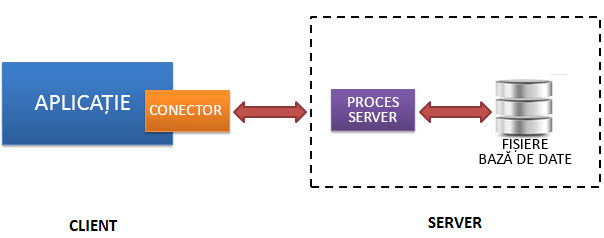
\includegraphics[width=0.9\textwidth]{Figures/client_server.jpg}}
  \caption{Arhitectura client-server a sistemelor de gestiune a bazelor de date relaționale}
\end{figure}

În figura de mai sus se poate observa arhictectura client/server unui sisteme de gestiune a bazelor de date relationale.
SQLite nu funcționează respectând aceste principii, acesta neavând necesitatea folosirii unui server pentru a rula.
Baza de date SQLite este întegrată în cadrul aplicației ce o accesează. Aplicația interacționează cu direct cu baza de date stocată local.

\begin{figure}[h!]
  \centering
    \centering{%
      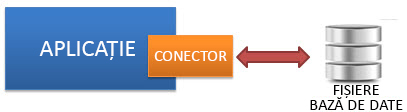
\includegraphics[width=0.7\textwidth]{Figures/sqlite.jpg}}
  \caption{Arhitectura server-less SQLite}
\end{figure}

\subsection{Independența}
Proprietatea de independență se definește prin necesitatea minimă de susținere din partea sistemului de operare sau a unei biblioteci externe. Aceasta îi acordă SQLite-ului avantajul de a rula în orice tip de mediu, în mod deosebit dispozitivele embedded precum iPhone, Android, console de jocuri, ș.a.m.d.
\vspace{6pt}
\\SQLite este dezvoltat folosind \acrshort{ansi}-C. Codul sursă este disponibil sub forma unui fișier sqlite3.c și header-ul atribuit acestuia, sqlite3.h. Dacă se dorește dezvoltarea unei aplicații folosind SQLite nu este necesară decât simpla adaugare a acestor fișiere în proiectul respectiv și compilarea codului.

\subsection{Zero-configurare}
Datorită arhitecturii ce nu include server, nu este necesară nici o instalare a SQLite-ului anterior folosirii sale. Nu exită nici un process de server ce necesită configurare, pornire sau oprire.
\vspace{6pt}
\\În plus, SQLite nu folosește nici un fișier de configurare.

\subsection{Tranzacțională}
Toate tranzacțiile din cadrul SQLite sunt conforme ACID. Acest lucru înseamnă că toate interogările și schimbările sunt Atomice, Consistente, Izolate și Durabile.
\vspace{6pt}
\\În alte cuvinte, toate schimbările ce apar în urma unei tranzacțiii sunt fie realizate în totalitate, fie deloc, chiar și în situații neprevăzute precum închidere neașteptată a aplicației, probleme de alimentare, sau probleme datorate sistemului de operare.

\subsection{Caracteristici specifice ale SQLite}
SQLite folosește tipuri dinamice pentru tabele. Acest lucru înseamnă că se pot stoca orice valori în orice coloane, indiferent de tipul de tipul de dată.
\vspace{6pt}
\\De asemenea, SQLite oferă libertatea ca o singură conexiune să acceseze simultan mai multe fișiere ale bazei de date. Acestă caracteristică este foarte facilă mai ales atunci când dorim să unim tabele din baze de date diferite sau să copiem date între baze de date diferite folosind o singură comandă.


\section{Structura bazei de date}

\begin{figure}[h!]
  \centering
    \centering{%
      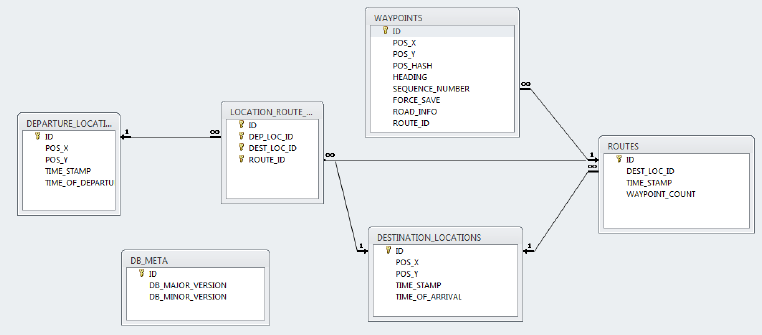
\includegraphics[width=0.9\textwidth]{Figures/baza_date.png}}
  \caption{Structura tabelelor de date şi relaţiile dintre ele}
\end{figure}

Tabelele din figura de mai sus sunt folosite pentru realiza structura întregii baze de date.
\vspace{6pt}
\\Tabela meta este folosită la identificarea versiunii bazei de date. Acest lucru este necesar pentru a detecta compatibilitatea şi pentru a permite migrarea către o versiune mai recentă. 
\vspace{6pt}
\\Datele înregistrate sunt separate în puncte de plecare, destinaţii, rute şi waypoint-uri. O rută este întotdeauna formată din mai multe waypoint-uri, unul sau mai multe puncte de plecare şi una sau mai multe destinaţii. Ruta (waypoint-urile) sunt stocate numai o singură dată, în timp ce toate punctele de plecare şi destinaţiile sunt stocate. În acest fel, numărul de destinaţii poate influenţa probabilitatea rutei.
\vspace{6pt}
\\Accesul la date se face prin SQLite. Toate datele stocate pot fi atât citite cât şi modificate.


